\documentclass[11pt]{beamer}
\usetheme{Dresden}
\usepackage[utf8]{inputenc}
%\usepackage[french]{babel}
\usepackage{hyperref}
\usepackage[T1]{fontenc}
\usepackage{amsmath}
\usepackage{amsfonts}
\usepackage{amssymb}
%\author{}
\title{La télédétection : fonctionnement et applications}
%\setbeamercovered{transparent} 
\setbeamertemplate{navigation symbols}{} 
\logo{} 
%\institute{} 
%\date{} 
%\subject{} 
\begin{document}

\begin{frame}
\titlepage
\centering

\includegraphics[scale=1]{img/logos.jpg}
\end{frame}

\begin{frame}
\tableofcontents
\end{frame}

\section{Qu'est ce que la télédétection ?}
\subsection{Définition}
\begin{frame}{}
\begin{itemize}
\item « l’ensemble des connaissances et techniques utilisées pour déterminer des caractéristiques physiques et biologiques d’objets par des mesures effectuées à distance, sans contact matériel avec ceux-ci » (COMITAAS, 1988)
\item Appareils :
\begin{itemize}
\item satellite
\item avion
\item drone
\end{itemize}
\end{itemize}
\end{frame}

\subsection{Acquisition d'informations}
\begin{frame}{}
\begin{itemize}
\item Spectre électromagnétique
\begin{figure}[!h]
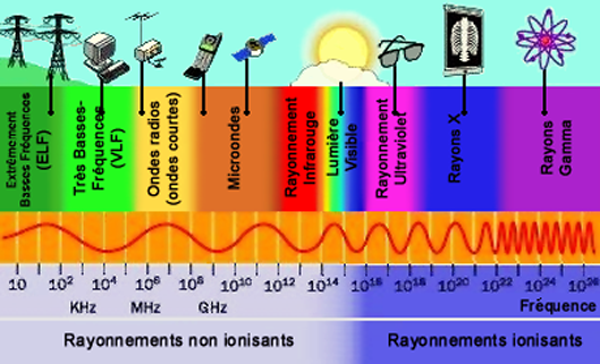
\includegraphics[scale=0.40]{img/spectre-electromagnetique.png}
\caption{Représentation du spectre électromagnétique (source : astronoo.com)}
\label{spectreElectro}
\end{figure}
\end{itemize}
\end{frame}

\subsection{Types de capteurs}
\begin{frame}{}
\begin{itemize}
\item Optique
\begin{itemize}
\item enregistre le rayonnement électromagnétique (appareil photo)
\end{itemize} 
\item Radar
\begin{itemize}
\item envoie un signal dans les micro-ondes et enregistre le retour (mesure)
\item capable de traverser les nuages, couverts forestiers, sols sous certaines conditions
\end{itemize} 
\item Laser
\begin{itemize}
\item envoie un laser et enregistre le retour (mesure)
\end{itemize} 
\item nombreux satellites avec différents instruments, résolutions, coûts, objectifs, applications, etc...
\end{itemize}
\end{frame}

\section{Interaction spectre électromagnétique <-> biosphère}
\subsection{Capteurs optiques : visible et proche infrarouge}
\begin{frame}{}
\begin{figure}[!h]
\centering
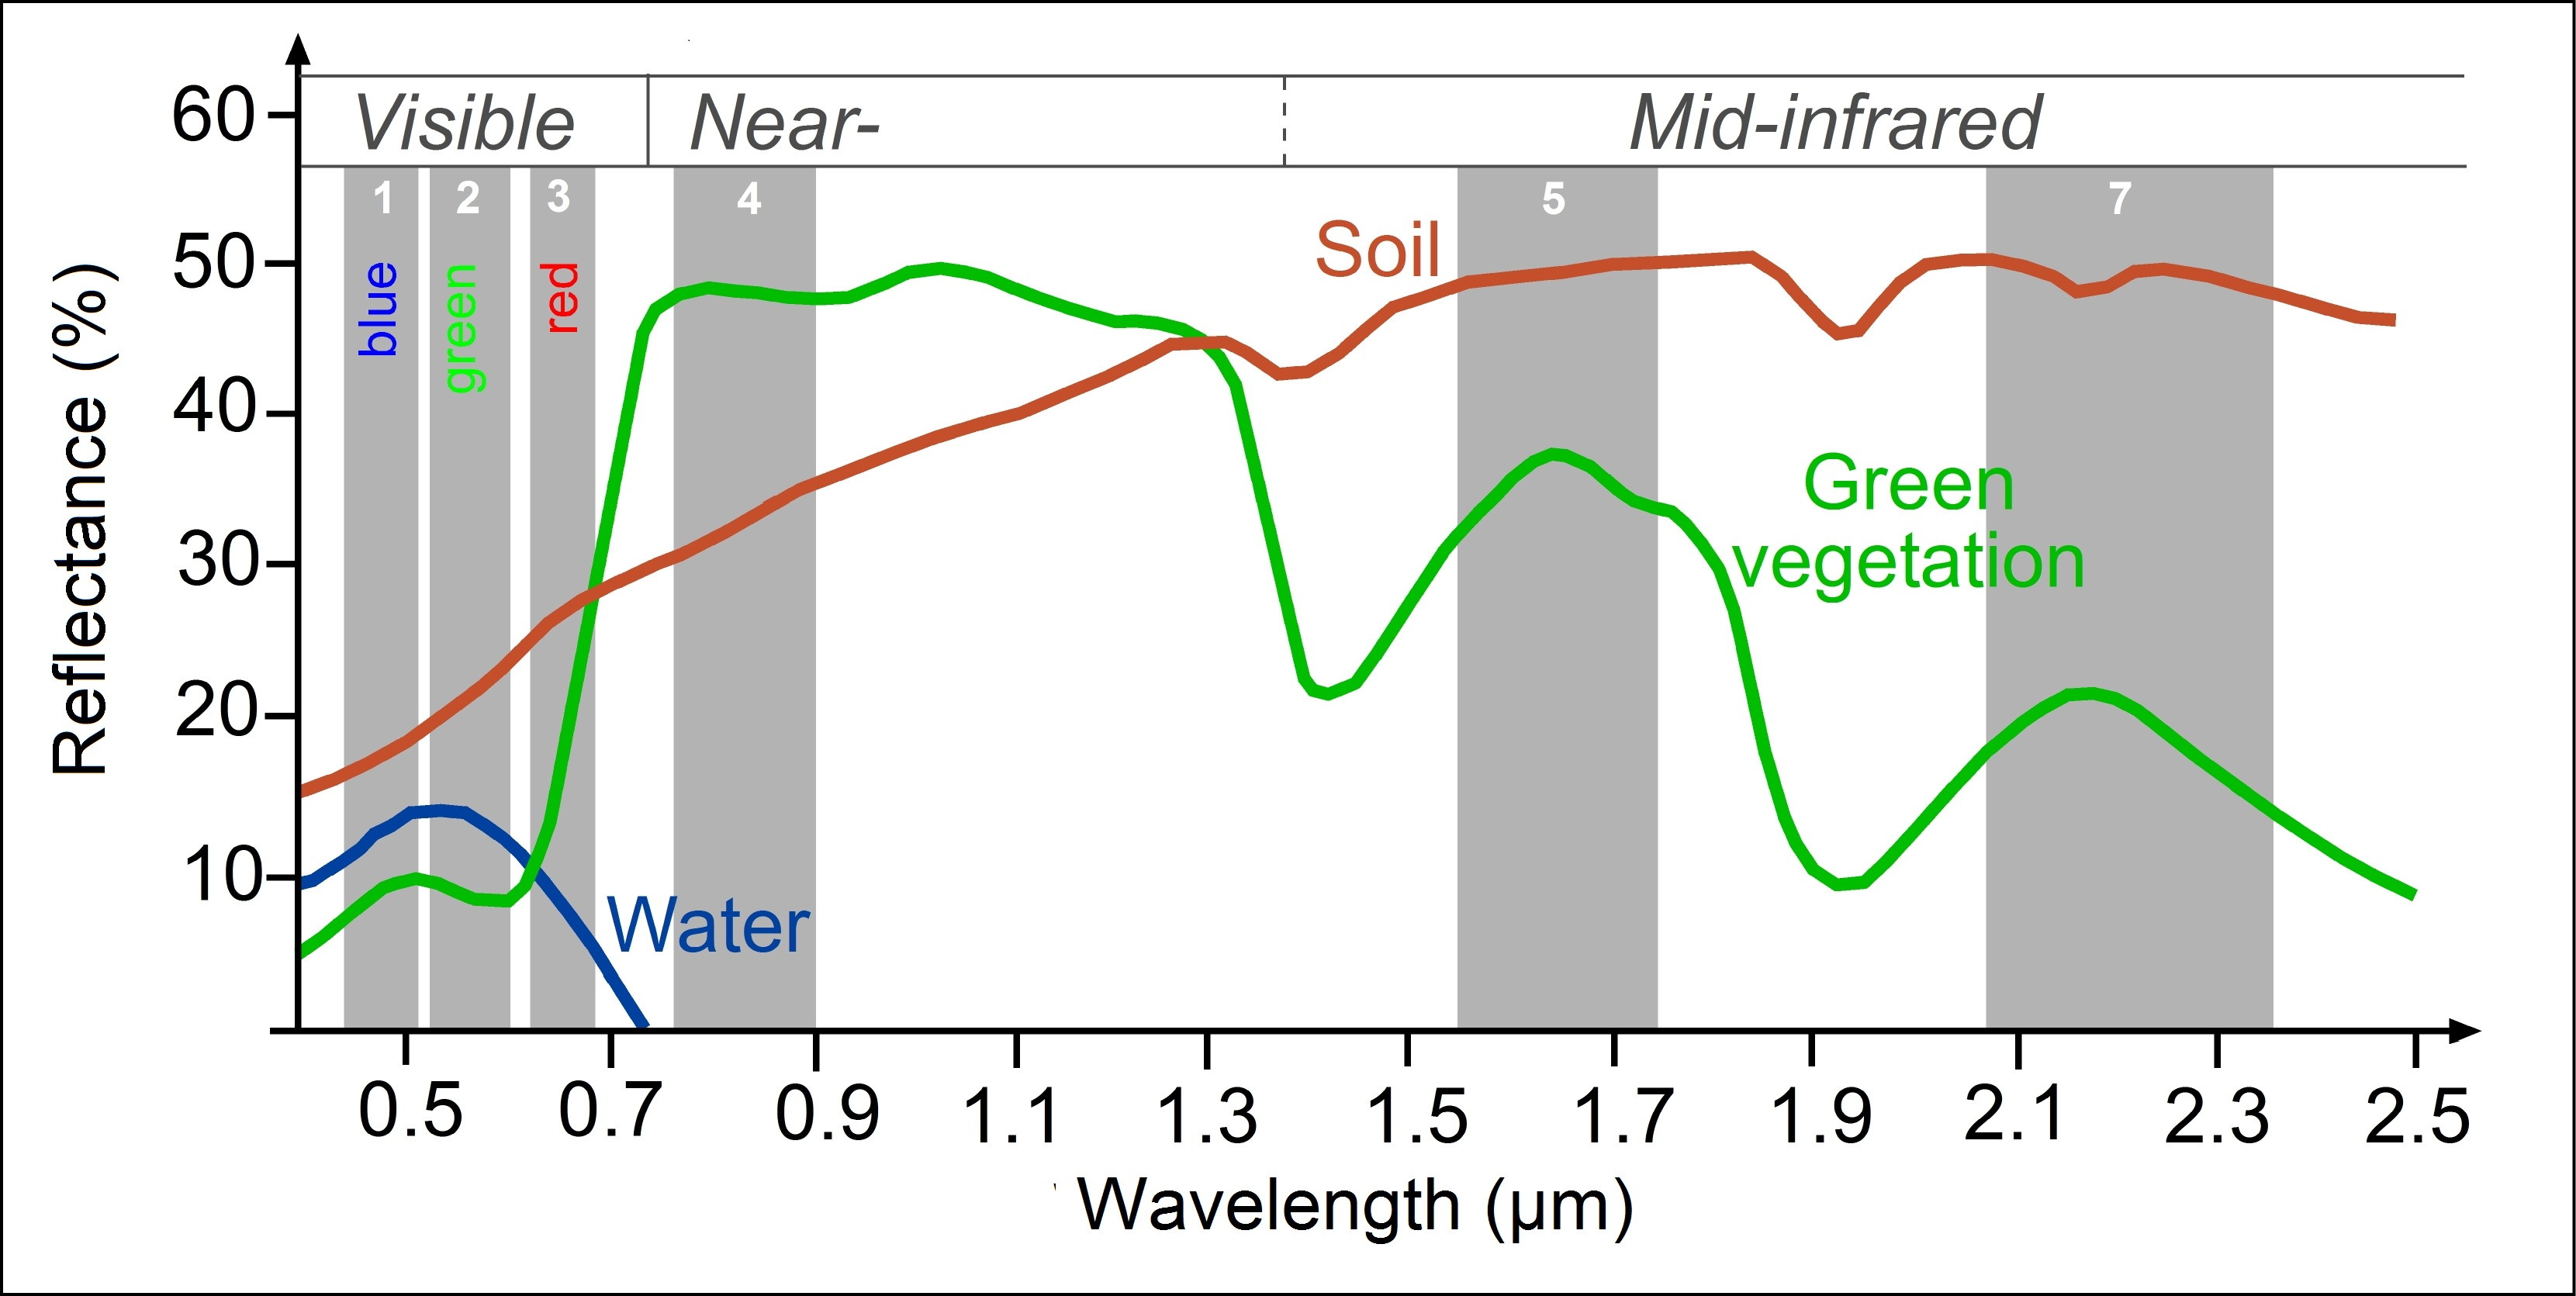
\includegraphics[scale=0.38]{img/spectral_signatures.jpg}
\caption{Signatures spectrales du sol, de l'eau et de la végétation vis à vis du spectre électromagnétique entre 350 et 2500nm. Source: SEOS Project}
\label{signSpectr}
\end{figure}
\end{frame}

\begin{frame}{}
\begin{figure}[!h]
\centering
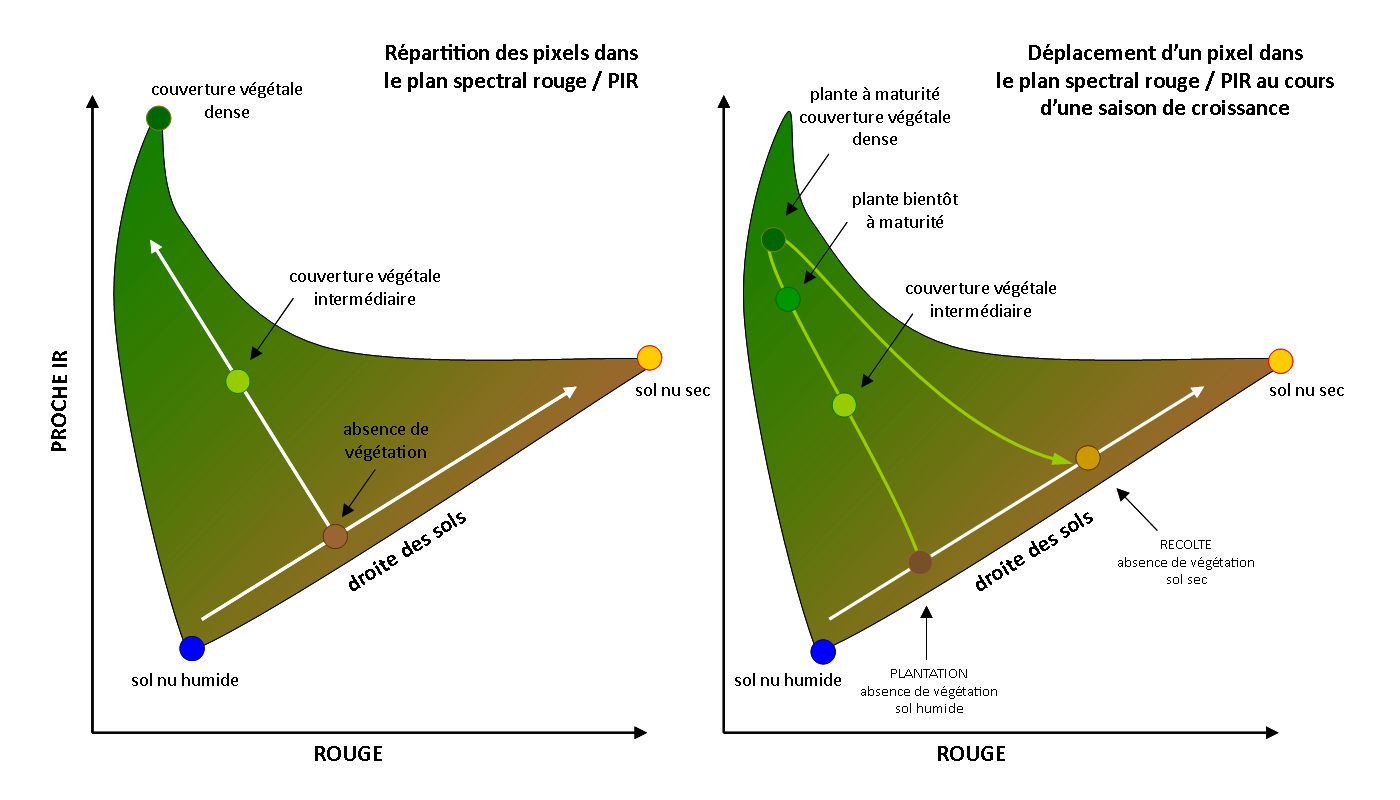
\includegraphics[scale=0.45]{img/droite_sols.png}
\caption{Droite des sols. Crédit : Copyright 2010 © The University of Arizona (Jensen, 2000)}
\label{signSpectr}
\end{figure}
\end{frame}

\subsection{Capteurs radars}
\begin{frame}{}
\begin{figure}[!h]
\centering
\begin{minipage}[c]{.46\linewidth}
      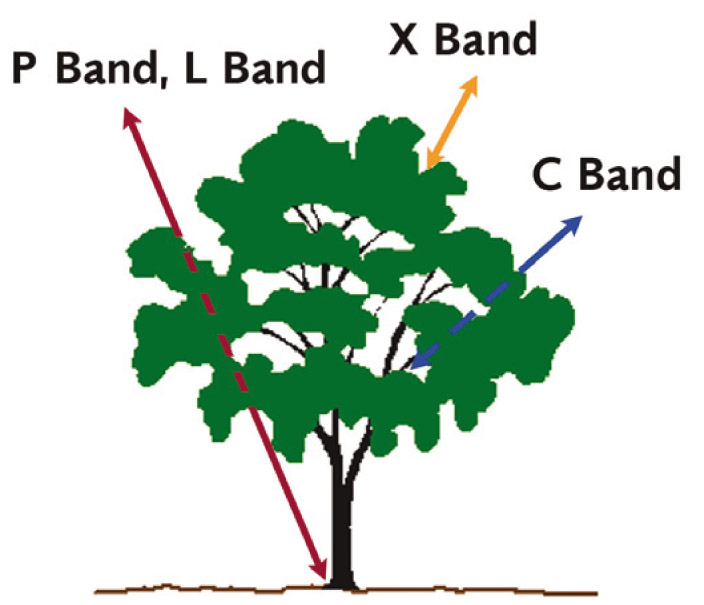
\includegraphics[scale=0.45]{img/radar_band.jpg}
      \caption{Interaction des bandes radar avec les forêts}
   \end{minipage} \hfill
   \begin{minipage}[c]{.46\linewidth}
      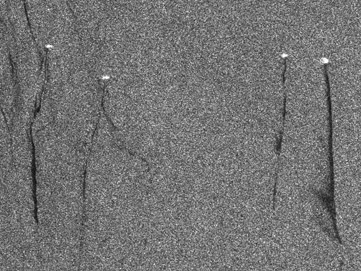
\includegraphics[scale=0.4]{img/radar-pollution.jpg}
      \caption{Détection de bateaux et d'opérations de dégazage. Source : CLS}
   \end{minipage}
\end{figure}
\end{frame}

\subsection{Capteurs lasers}
\begin{frame}{}
\begin{figure}[!h]
\centering
\begin{minipage}[c]{.46\linewidth}
      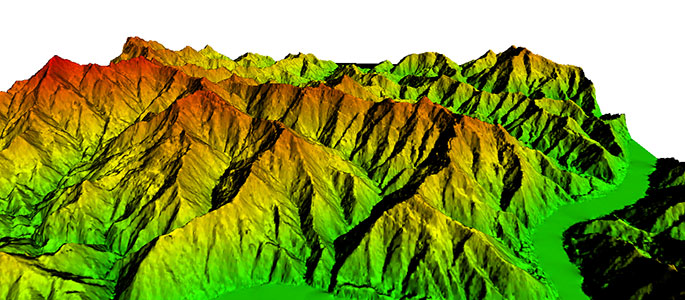
\includegraphics[scale=0.22]{img/lidar_dem.jpg}
      \caption{Modèle Numérique de Terrain (MNT) réalisé à partir de mesures LIDAR.}
   \end{minipage} \hfill
   \begin{minipage}[c]{.46\linewidth}
      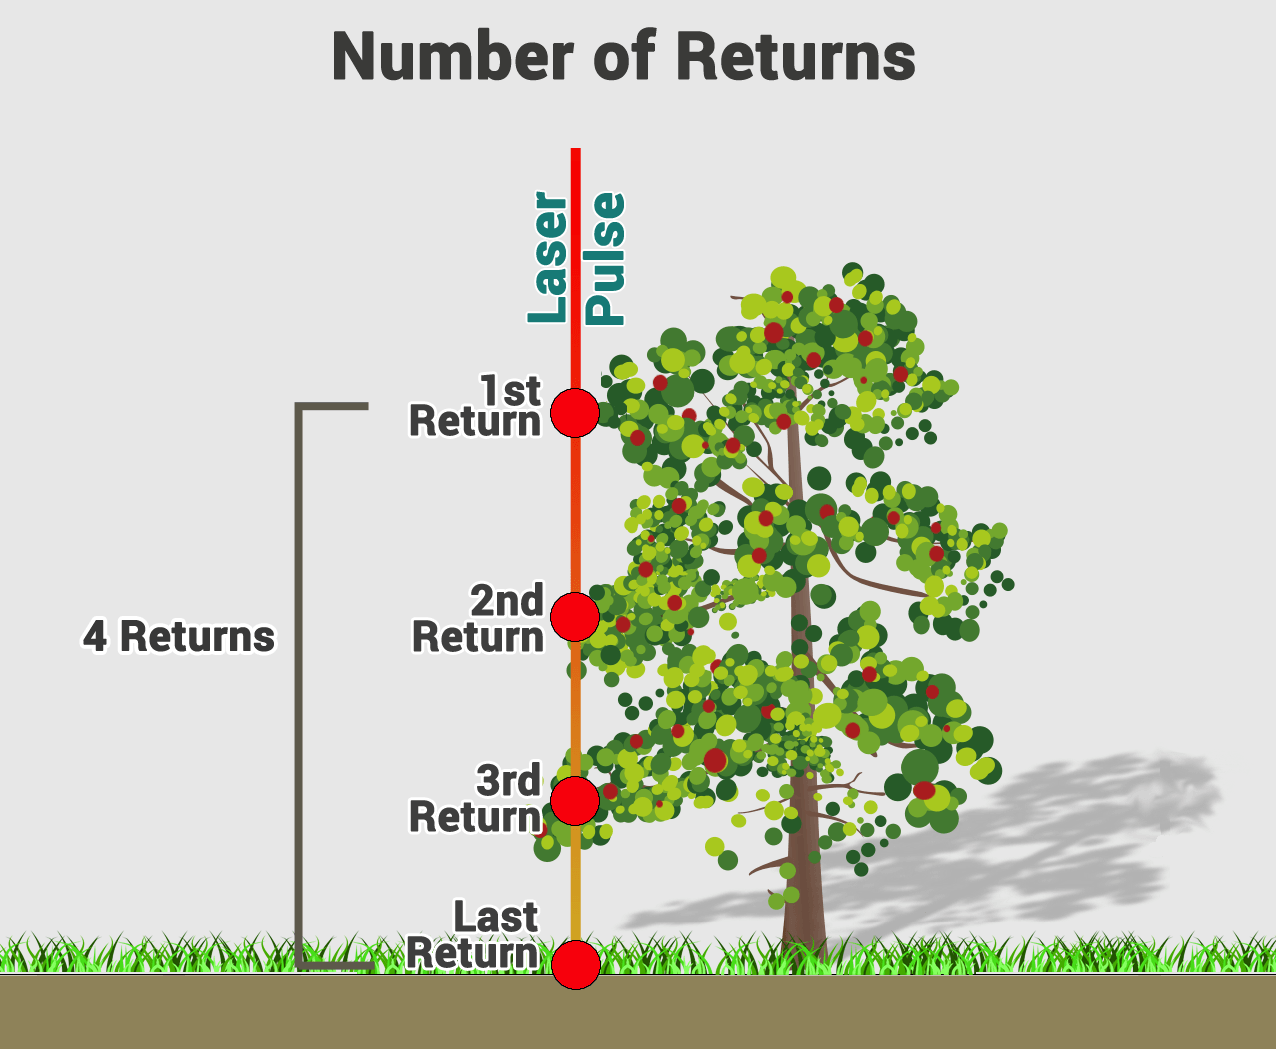
\includegraphics[scale=0.11]{img/lidar_modelisation.png}
      \caption{Utilisation du LIDAR pour modéliser une forêt. Source : GIS Geography}
   \end{minipage}
\end{figure}
\end{frame}

\section{Au delà du spectre}
\subsection{Néo-canaux}
\begin{frame}{}
\begin{itemize}
\item Indices de végétation pour étudier la végétation (croissance, état sanitaire, stress hydrique) et l'occupation du sol (forêt, prairie, sol, eau).
\item Indices pour étudier le sol (composition, humidité, rugosité, structure)
\item Indices pour étudier les zones en eau libre (taux de nutriments, épaisseur de la lame d'eau)
\item Bien d'autres...
\end{itemize}
\end{frame}

\subsection{Temporalité}
\begin{frame}{}
\begin{itemize}

\item Phénologie : suivi et distinction de l'usage ou d’événements
\begin{figure}[!h]
\centering
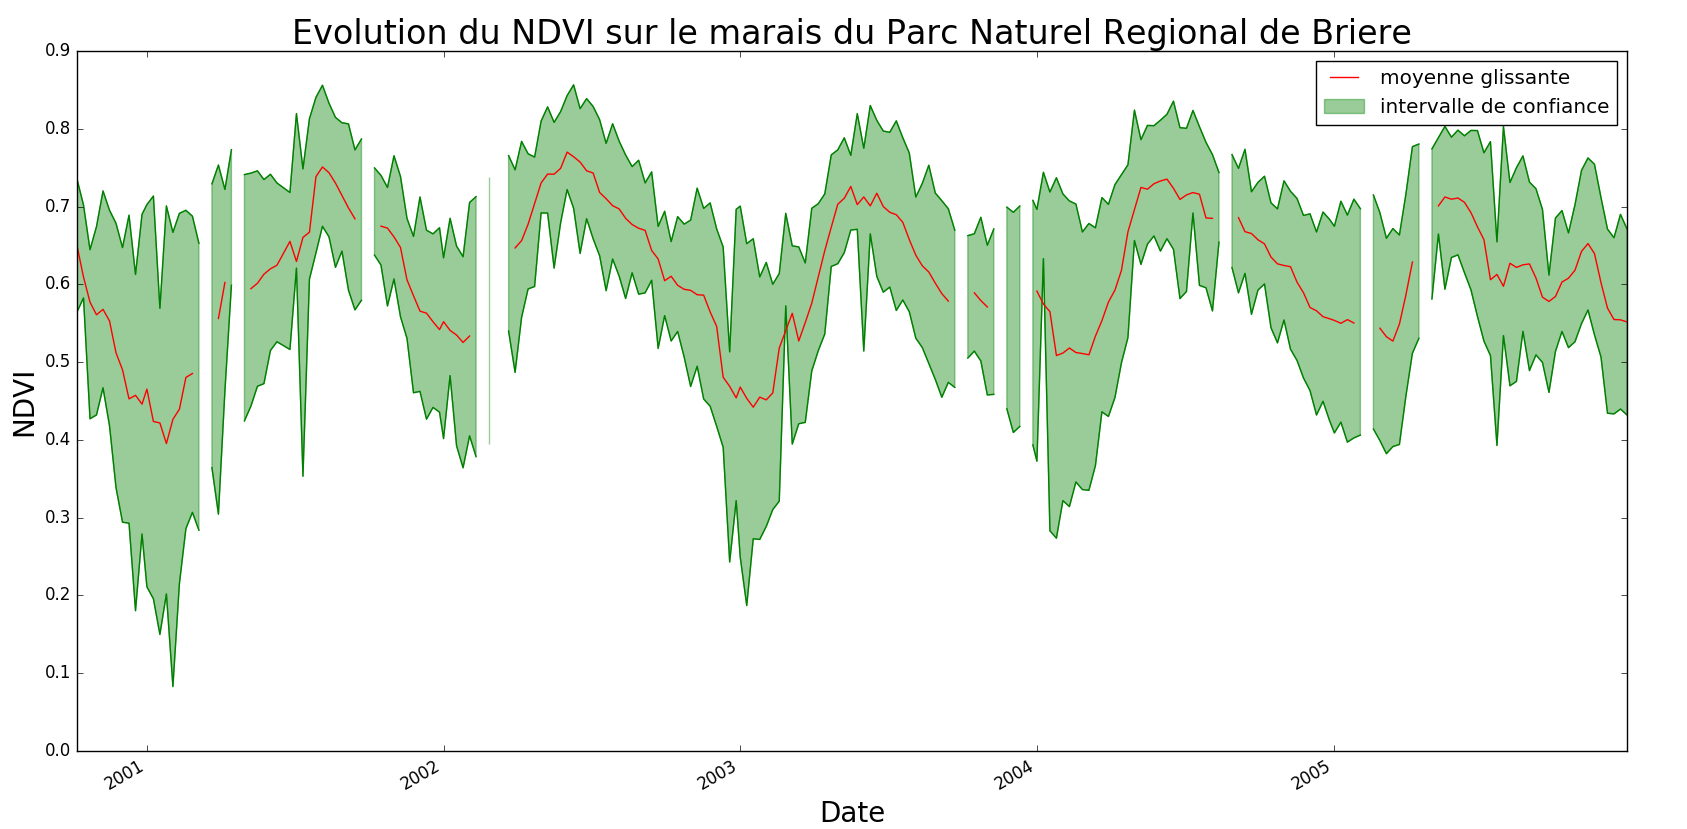
\includegraphics[scale=0.22]{img/NDVI_Briere.png}
\end{figure}
\item Urbanisation : emprise urbaine, effet d'un barrage hydraulique
\item Aléa : image pré et post-événement (tempête, inondation, réchauffement climatique)
\end{itemize}
\end{frame}

\subsection{Classification}
\begin{frame}{}
\begin{itemize}
\item simplifier l'analyse d'une image
\begin{figure}[!h]
\centering
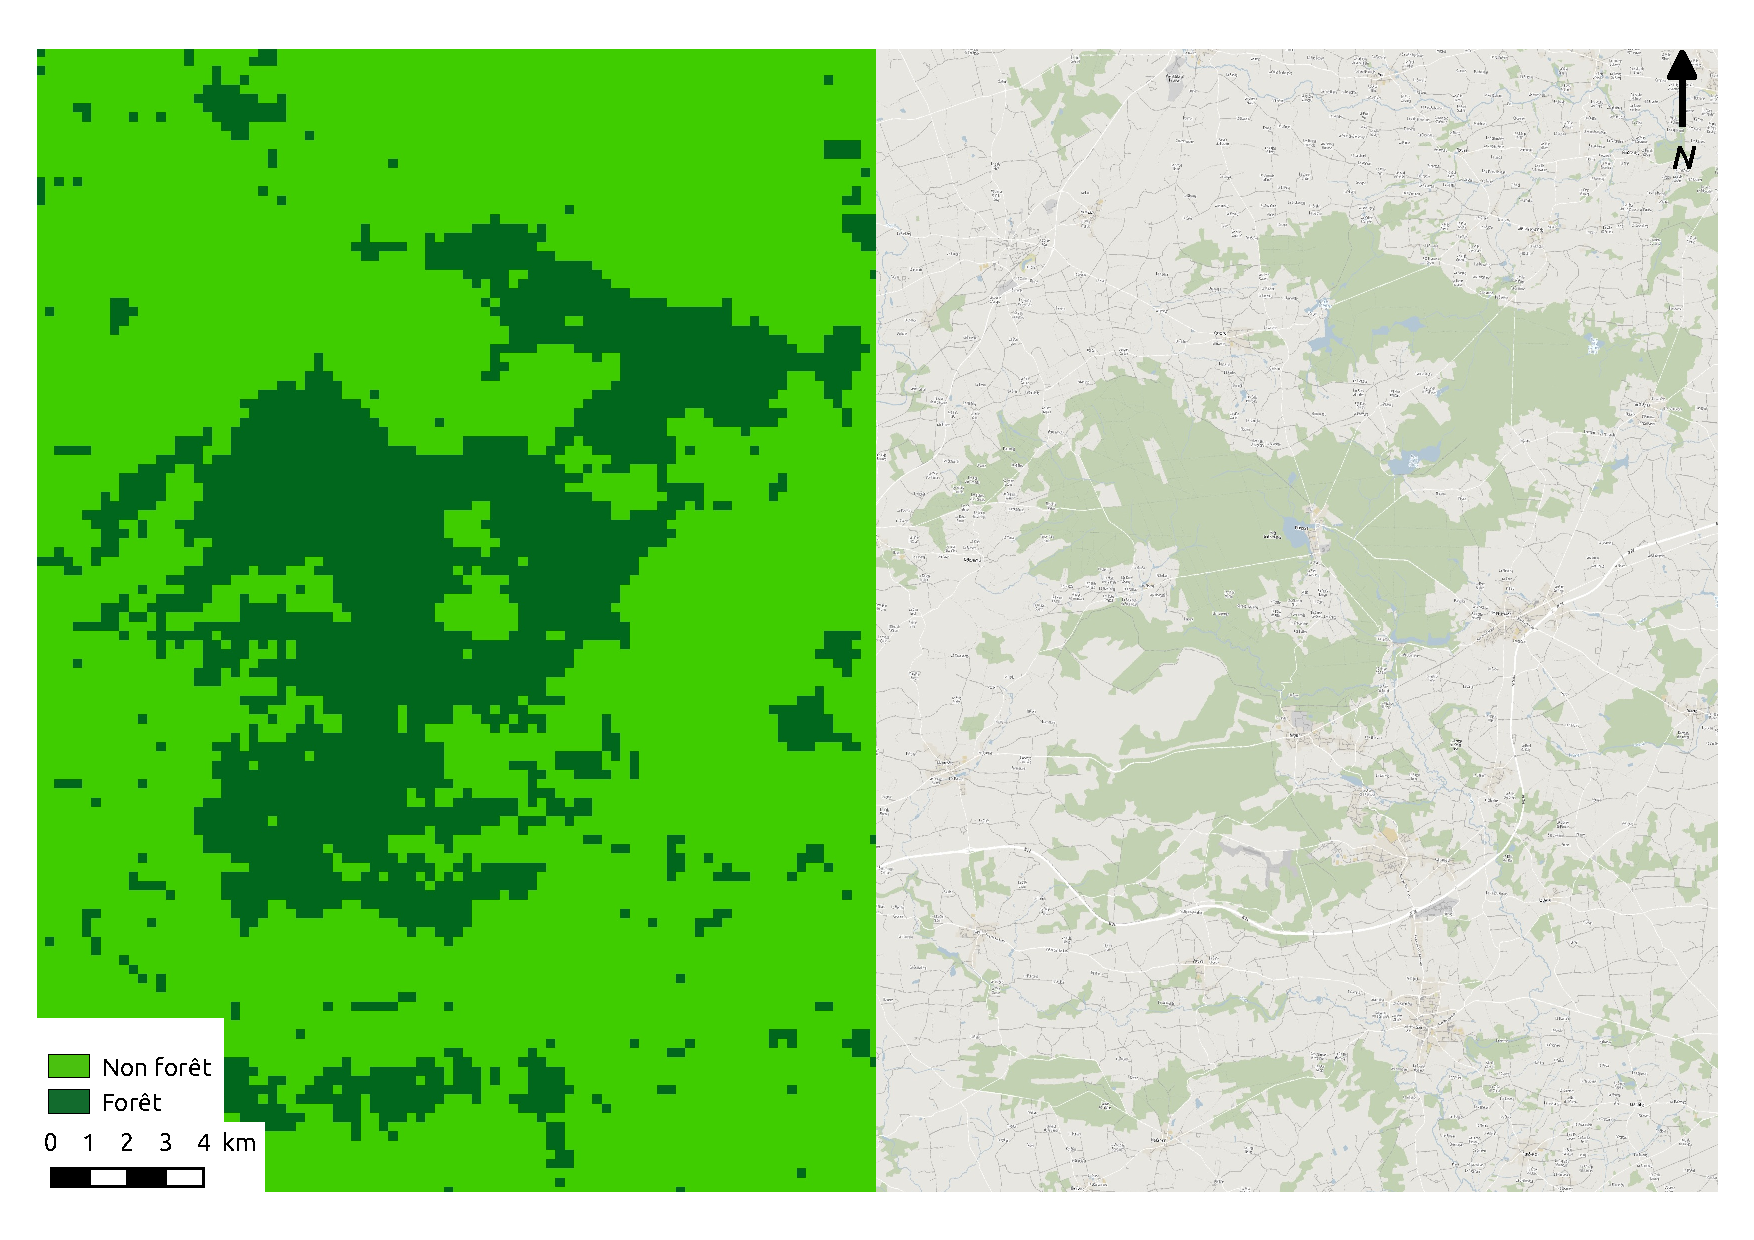
\includegraphics[scale=0.29]{img/classif_exemple.pdf}
\end{figure}
\end{itemize}
\end{frame}

\begin{frame}{}
\begin{itemize}
\item permettre l'utilisation d'outils (métriques paysagères)
\begin{figure}[!h]
\centering
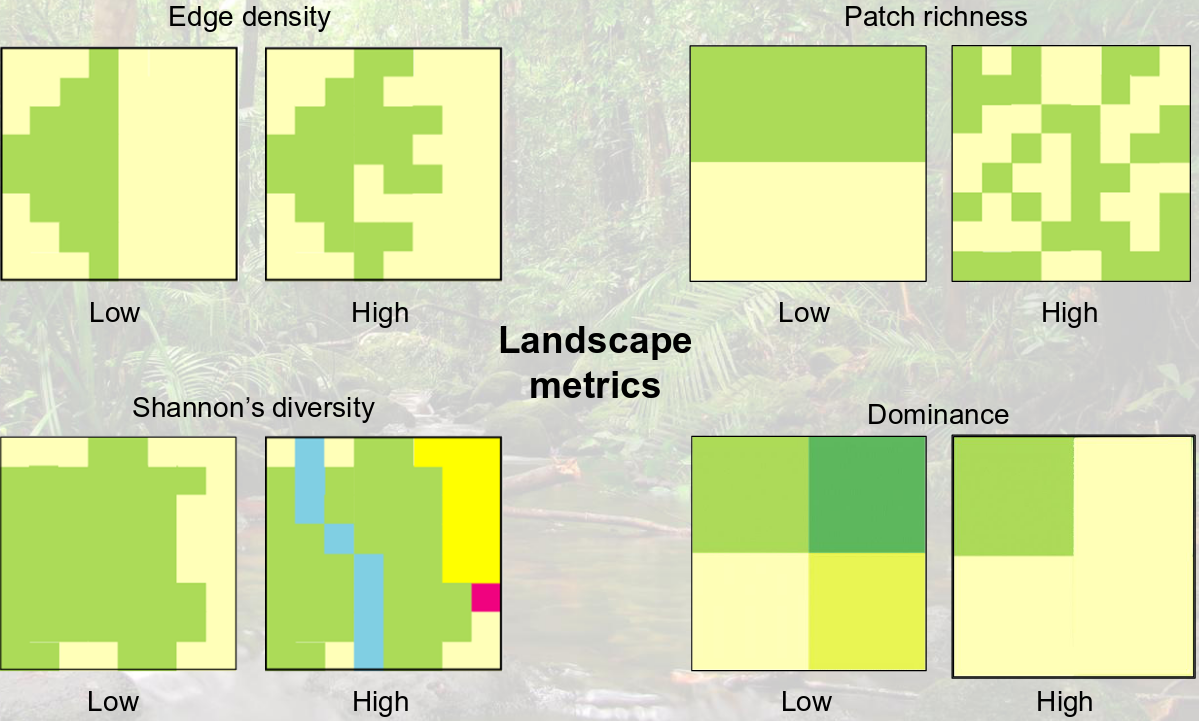
\includegraphics[scale=0.22]{img/metrique_paysage.png}
\end{figure}
\end{itemize}
\end{frame}

\section{Conclusion}
\begin{frame}{}
La télédétection :
\begin{itemize}
\item est un domaine permettant d'acquérir de nombreuses informations
\item permet d'acquérir des informations de manière continue et à moindre coût (enquête terrain)
\item s’intègre dans de nombreuses thématiques (urbanisme, défense, écologie, océanographie, etc...)
\item fonctionne parfaitement avec les standards OGC/INSPIRE \url{http://geowww.agrocampus-ouest.fr/sviewer/?wmc=e876c9ade943853da0cbca26ea6823f5}
\end{itemize}
\end{frame}

\begin{frame}{}
\centering Fin

\includegraphics[scale=1]{img/logos.jpg}
\end{frame}

\end{document}